\chapter[SCP-001 世界,收容失败]{
    SCP-001 BILLITH - The World at Large \\
    SCP-001 世界,收容失败
}

\label{chap:SCP-001.the.world.at.large}

\begin{scpbox}

\begin{center}

\Gg{\bb{\mono{您正在访问SITE-01归档文件}}}

\mono{深层存储}

\ii{\mono{请稍候……}}

\end{center}

\end{scpbox}

\begin{scpbox}

\ii{\mono{001.SCP.archive @ dir\slash arc\slash events\slash other\slash EE00059.rtf 加载中…}}

\mono{\bu{事件:}\uu{EE-00059}}

\bi{因EE-00059的性质,无须将其指定为一个SCP。EE-00059存在的情报基本上被认为是非异常的,因此目前不需要制定收容措施。在EE-00059附近发生的任何信号播送和活动都应上报并尽可能从公众知识中清除。}

\bb{事件描述:}2016年1月4日,在距地球约160万光年的太空区域观测到超常事件00059。\footnote{这表明其初始起源距今约160万年。}NASA的深空网络卫星系统在三小时内检测到了它。

EE-00059-1是事件期间的一系列低频传输信号,来自EE-00059方向。考虑到无线电波的范围和速度,其很可能由异常广播设备发送以传输消息。(查阅\bb{EE-00059-1转录日志}以获取更多信息。)

EE-00059-2是一个新出现的E级“因果暂失”虫洞(S-CSMWAUC2-T)。\footnote{空间性,循环稳定,有形体,广域,非定性,条件双向,瞬态。更多信息请参阅:\ii{\hyperref[sec:DOC-about.black.hole]{统一技术设定论述,关于超维度出入口(即虫洞)的分级}}和其他\hyperref[chap:SCP-3989]{类似案例文件}。}EE-00059-2在EE-00059-1-3传输期间被观测到出现约102秒,同时表现出虫洞和白洞的性质,并喷射物质和光线,但对地球上常见的流体流动却有极大限制。这导致其异常可见度比普通情况大了几个数量级。在近距观察后,发现EE-00059-2并未表现出对周围重力有明显影响。这点与埃利斯虫洞更为符合,它是时空的非平坦三维区域之间的完全可转移点。

这种矛盾的表现意味着EE-00059-2是以我们自己的现实中不可能的手段创造的,该区域需要基金会进一步调查。

\end{scpbox}

\hr

\begin{scpbox}

\ii{\mono{00059.SCP.archive @ dir\slash arc\slash events\slash other\slash EE00059_Exploration.rtf 加载中…}}

\end{scpbox}

\begin{scpbox}
    
\begin{figure}[H]
    \centering
    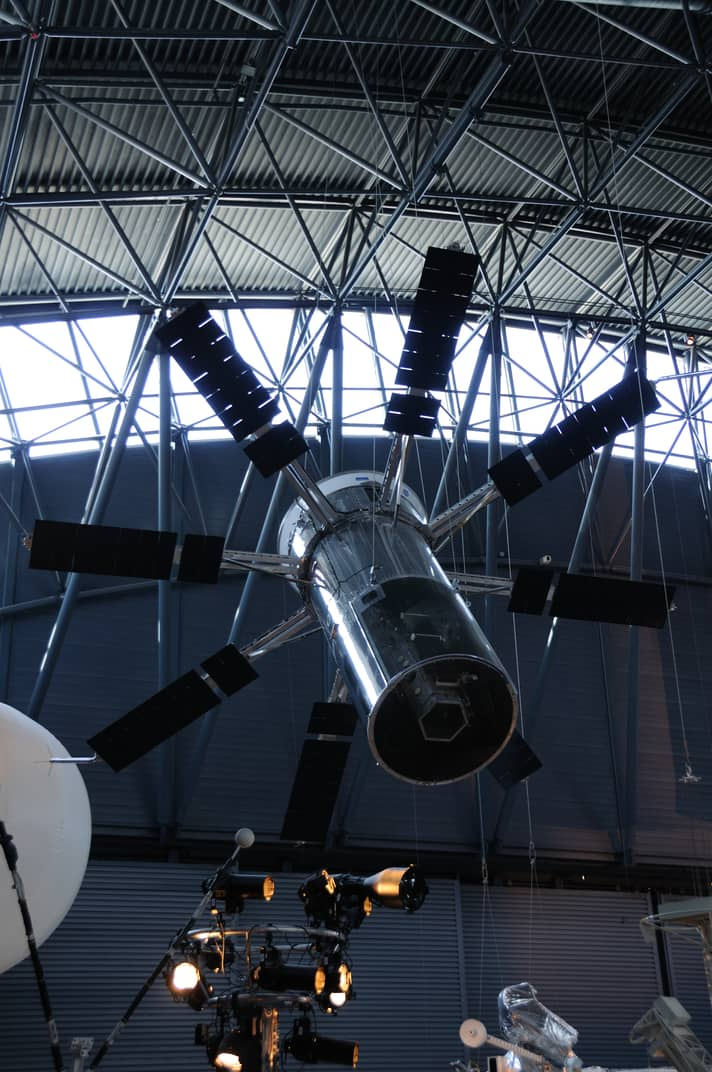
\includegraphics[width=0.5\linewidth]{images/SCP-001-the-world-at-large.jpg}
    \caption*{Altruist-9探测器,位于Site-88航空航天机库。}
\end{figure}

\bi{\mono{2027年5月18日,基金会提议建造Altruist-9深空探测器,以观察EE-00059所在区域的状况,O5议会以多数票通过。}}

为了在一定时间内到达指定地点,Altruist-9采用了超光速(FTL)驱动器和高效太阳帆。但是,由于灵敏度和探测器遭遇外空间异物的风险,超光速驱动引擎不会全功率工作。因此,Altruist-9预计在████年走完全程。

在EE-00059-2重现事件中,Altruist-9存放着一架小型太阳能无人机和一台大气测量设备的内核,被包裹在了一个外源的多肽低聚物编织结构中,物质来自\mono{{[}数据删除,见下]}的残骸。该物质推定是穿过EE-00059-2后存留了下来。Altruist-9于2038年1月8日发射。

\bb{更新:}

████年2月26日,即Altruist-9到达指定位置的时间,记录到的读数在开始是非异常的。然而,不久之后,就检测到了区域内的活动。EE-00059-2似乎在探测器附近重新打开了,并将探测器吸了进去。异常在102秒后关闭。

因白洞的反常和极端性质,Altruist-9可能无法在与EE-00059-2的接触中幸存。但推测探测器内核的功能性应该在穿越中保存了下来,并能够在EE-00059-2的另一侧进行观测,直到未来某天链接重建起来。

\end{scpbox}

\hr

\begin{scpbox}

\bi{\mono{001.SCP.archive @ dir\slash arc\slash events\slash other\slash EE00059-01_Log.rtf 加载中…}}

\tred{+ 访问00059-1-1转录日志}

\tred{确认}

00059-1-1转录日志

\ii{注意:这是从EE-00059方向接到的首次信号传输,持续了30分钟。上下文未知,只听到单方面讲话,标记为POI-00059-A。所有的传输信号使用的都是一种句法结构与英语类似的语言,因此可以相对容易地翻译。}

\hr

<开始转录>

\bb{POI-00059-A:} {[}静电噪声] -未知,也许他们能- {[}静电噪声]

\bb{POI-00059-A:} {[}静电噪声] -去,它不会落在后面太远。 

\bb{POI-00059-A:} 不,我不- {[}静电噪声]

\bb{POI-00059-A:} {[}静电噪声] -我们把它丢了。不确定。

\bb{POI-00059-A:} {[}无法拼出]

\bb{POI-00059-A:} 什么?十,三。是- {[}静电噪声]

\bb{POI-00059-A:} {[}静电噪声]

\bb{POI-00059-A:} 噢。噢不。

<转录结束>

\tred{+ 访问00059-1-2转录日志}

\tred{确认}

00059-1-2转录日志

\ii{注意:记录下的对话持续5分钟,应该发生于两方之间,标记为POI-00059-A和POI-00059-B。上下文未知。}

\hr

<开始转录>

\bb{POI-00059-A:} {[}静电噪声]

\bb{POI-00059-B:} {[}静电噪声]很匆忙,还是不知道什么时候- {[}静电噪声] -我们。

\bb{POI-00059-A:} 不需- {[}静电噪声] -那。我们的传感器正监测到反常{[}无法拼出]。

\bb{POI-00059-B:} 我们也是。你觉得这是- {[}静电噪声]

\bb{POI-00059-B:} 最好别深究。

\bb{POI-00059-B:} 收到了吗?十二,四。

\bb{POI-00059-A:}  只有- {[}静电噪声] -我们现在落单了。

\bb{POI-00059-B:} 那会多久?

\bb{POI-00059-A:} {[}静电噪声] -什么方法找到我们。

\bb{POI-00059-B:} {[}无法拼出]

<转录结束>

\tred{+ 访问00059-1-3转录日志(需00059或4级权限许可)}

\tred{确认}

00059-1-3转录日志

\ii{注意:这是EE-00059-2首次观测期间,从EE-00059方向收到的最后一段对话记录。此次对话持续10分钟,发生于两方之间,标记为POI-00059-A和POI-00059-B。}

\hr

<开始转录>

\bb{POI-00059-A:} {[}静电噪声] -一,四- {[}静电噪声] -一,八,收到请回复。

\bb{POI-00059-B:} 收到,你们需要离开。立刻。

\bb{POI-00059-A:} {[}静电噪声] -跳跃,二十- {[}静电噪声] -重复,二十秒差距。无法- {[}静电噪声] 十五。恒星体依然- {[}静电噪声]

\bb{POI-00059-B:} {[}静电噪声] -得马上离开这,马上!

\bb{POI-00059-A:} 等等,我们发现了- {[}静电噪声]

\bb{POI-00059-A:} 你们能听到吗,我们- {[}静电噪声]

\bb{POI-00059-B:} 是的,我们看到了。接着怎么办?

\bb{POI-00059-A:} {[}无法拼出]

\bb{POI-00059-B:} {[}静电噪声] -太草率了,很可能承受不住- {[}静电噪声]

\bb{POI-00059-A:} {[}静电噪声] -抱歉,Graham。{[}静电噪声] -驱动引擎没法及时就绪了。我觉得这是我们唯一的选择,否则我们必死无疑。

\bb{POI-00059-A:} {[}未知] -靠近了。告诉- {[}静电噪声] -他们。

\bb{POI-00059-B:} 一路平安。

\bb{POI-00059-A:} {[}静电噪声]这。好的我们几乎- {[}静电噪声]

\bb{POI-00059-B:} 什么?你们看见了什么?

\bb{POI-00059-A:} {[}无法拼出]

\bb{POI-00059-B:} 鹦鹉螺号,请重复。二十,四。

\bb{POI-00059-A:} {[}尖叫]

\bb{POI-00059-B:} {[}静电噪声] -螺号!我们得移动- {[}静电噪声] -也许损失- {[}静电噪声]

\bb{POI-00059-B:} 那东西消失了。它去哪儿了?在哪 -{[}静电噪声]

\bb{POI-00059-B:} {[}静电噪声]

\bb{POI-00059-B:} 这里是天命号舰长Graham Ereshkigal,隶属人类████████星系运输船队。如果有人收到,这是我们的最后讯息,地球它,它不见了。我们不确定及时- {[}静电噪声] -能否。我们在Laniakia,或许- {[}静电噪声] -救援,我不知道。我不知道。

\bb{POI-00059-B:} 我们必须进入超光速,但告诉- {[}无法拼出] 

\bb{POI-00059-B:} {[}静电噪声]

<转录结束>

\end{scpbox}

\hr

\begin{scpbox}

\bi{\mono{05.001.SCP.archive @ dir\slash arc\slash mainlist\slash SCP-001.rtf 加载中…}}

\end{scpbox}

\begin{scpbox}

\begin{figure}[H]
    \centering
    
\includegraphics[width=0.5\linewidth]{images/SCP-001-the-world-at-large-2.jpg}
    \caption*{SCP-001}
\end{figure}

\bb{项目编号:}SCP-001

\bb{项目等级:}Netzach 

\bb{特殊收容措施:}N\slash A

\bb{描述:}SCP-001是所谓地球的行星体的名称。鉴于SCP-001养育了人类的整个文明,与基金会深空计划所观察到的视界宇宙内其他行星相比,地球的异常不可能性被公众广泛认为是“正常”的。

SCP-001-E1是1956年在智利安托法加斯塔地区阿塔卡马沙漠进行考古探险时发现的航天器残骸的名称,看上去已经被改造为临时生存空间。飞船的残余部分由外源的未知组分高耐久合金构成,材料的年代测定结果也不一致。尽管如此,回收到的材料表明飞船已有数百万年历史。

衣物,电子产品和家具等物品的残余也已收回,所有物品都含有不同程度抗正常磨损的异常材料。飞船的全尺寸未知但据信足够大以能容纳中等数量的人类,除了从SCP-001-E2内部回收的POI-001外,其余残留物均已自然分解。

SCP-001-E2是一组\dd{32} 36个高度先进的低温休眠舱,是挖掘SCP-001-E2时,于一块以部分“冬眠”模式供能的残骸中发现的。在所有发现的舱室中,只有一个仍然在运作并且含有\mono{{[}应监督者要求删除]},该生命体的宗旨使得基金会之后在地球上建立起来。

\end{scpbox}

\begin{figure}[H]
    \centering
    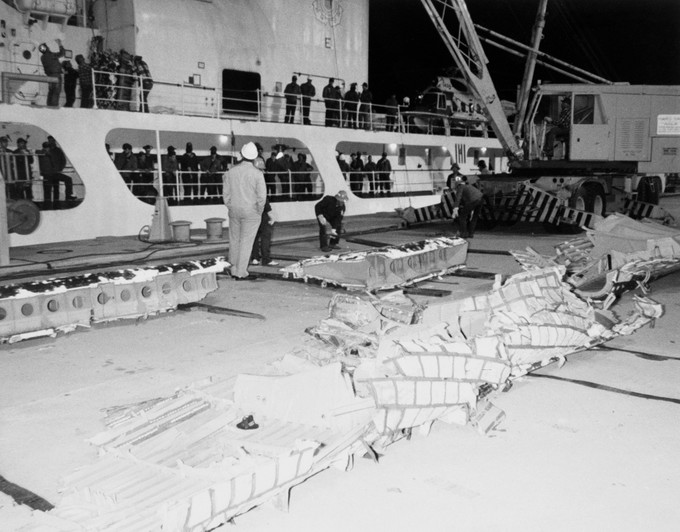
\includegraphics[width=0.5\linewidth]{images/SCP-001-the-world-at-large-3.jpg}
    \caption*{残骸从智利西海岸运离,1957年。}
\end{figure}

\begin{scpbox}

在瓦砾中有几个完全损毁的数据存储设备,目前唯一恢复出的信息片段是一张1cm x 1cm的磁盘碎片,由异常材料构成。已知该材料是一种高度压缩的多层信息介质,呈现为一组垂直堆叠数据的薄层结构。下面是从数据中恢复出的文档,由他们的原始语言翻译而来,这是一组I类认知危害型文字,其性质使得尽管对该语言的理解和阅读水平都很有限,读者仍然能够100%理解材料。对语言的分析正在进行中。

\hr

\tred{访问 001-E1-a89.rtf }

\tred{- 关闭}

\mono{\bb{修订版本:A.89}}

\mono{\bb{分类:神经学}}

\mono{\bb{详情:当前认为A.89行为复合体的实施方案很成功,不需要进一步改动。如果未来出现VIII级大气危害情景,将立即修改和实施A.89策略,以最大限度地减少伤亡并将新的人形生命形式纳入适当的宿主环境。}}

\mono{\bb{A.89行为复合体于124.5, 8.4M实施,在类地的陆地行星AXIOM-8上成功进行了宿主整合。}}

\mono{\bb{在主地球被太阳撞击破坏后的人口迁移行动中,AXIOM-8被认为最适合人形生命生存。已接触AXIOM-8并证实其无人居住并含有氮为主的大气。}}

\mono{\bb{由于VIII类大气危害情景中AXIOM-8被大约21%体积的高腐蚀性O\textsubscript{2}污染,基础设施和人类收容\slash 生活区域的建立进程中断,并且其对大多数生命形式有致命危害,需要实施A.89。}}

\mono{\bb{A.89是一套条件反射和对基础生理学的修改,使用泛星系基金会的\hyperref[chap:SCP-2000]{生物进化诱导器}(BECM)改变了产生的新生命形式的一般生物学特性。A.89的主要复合体是一种下意识的振荡行为,包括短时间吸​​入空气,随后扩张鼓膜,合理平衡周围环境的超压力,并缓解大气中小规模的氮流失及氧的暂时性危险失衡。此外,也正在进行小幅改造,以使得氧气能够成为支持广泛生命的物质。研究正进行中。}}

\mono{\bb{附录:实验记录}}

\mono{\bi{以下为使用泛星系基金会生物进化诱导器(BECM)对应用A.89的生命形式进行各种测试的简要总结。}}

\begin{longtable}{m{0.2\linewidth}m{0.2\linewidth}m{\0.5\linewidth}}
\hline
测试编号 & 生命形式 & 结果\\
\hline
\endhead
\hline\multicolumn{3}{r}{\small{接下页}}
\endfoot
\hline
\endlastfoot
A.89-1 & 主地球爬行动物(小) & 应用失败。暴露于AXIOM-8会导致由于压力变化和细胞快速氧化发生的大出血。\\
A.89-2 & 主地球爬行动物(小) & 应用失败。当试图利用新的生理学改变时,受试体死于癫痫发作。为了完善该点需重新调整神经连接通路。\\
A.89-8 & 主地球爬行动物(大) & 应用部分成功。受试体在暴露于AXIOM-8两个周期后才死于细胞氧化,比平时更长。A.89行为似乎可以防止氮剥夺;进行了脂质测量,结果正常。\\
A.89-15 & 主地球爬行动物(大) & 应用部分成功。暴露未导致压力失衡,整个过程中都出现了A.89行为。由于氮剥夺,试体不久后陷入昏迷。\\
A.89-22 & 主地球爬行动物(大) & 应用部分成功。生理适应性失控。受试体表现出抗处决性,在受到损伤后通常以惊人速度恢复。受试体目前关押于高安全收容室留待进一步研究。\\
A.89-27 & 标准人类 & 应用成功。受试体能够承受AXIOM-8的大气。观察到轻微头痛和偶发鼻出血。\\
A.89-38 & 五(5)标准人类 & 应用部分成功。除非聚在一起,否则受试体能够承受AXIOM-8大气。当存在多种生命形式时,特别高密度的氧气仍会导致氮剥夺。\\
A.89-40 & 五(5)标准人类 & 应用部分成功。在群体中施用轻度认知影响以启动A.89可显着降低死亡率。对正在进行的氮气总量要求进行了基础修改,但这些计划在12个周期以后才会完成。\\
A.89-44 & 五(5)标准人类 & 应用成功。97.8%的个体通过认知效应成功避免死亡。正在努力将人类的平均寿命延长回至███。\\
A.89-68 & 一标准人类 & 应用部分成功。细胞氧化扼制足以使平均寿命延长至██,是之前平均值的五倍。对生理学的进一步改造不会有额外增益。
\end{longtable}

\tred{访问 001-E1-axiom.rtf}

\tred{- 关闭}

\mono{\bu{AXIOM-8}}

\mono{\bb{毫无疑问,人体是一个难解之谜。经过数千年的休眠,对新家园的上下求索将我们最终引向了一个与主地球有着惊人相似之处的星球。这是最大的谜团。}}

{[}数据损坏]

\tred{访问 001-E1-note.rtf}

\tred{- 关闭}

{[}数据损坏]

\mono{\bb{能经得起时间的考验,如果你发现了它,而我们已不再存在,或者我们忘记了我们是谁,我们来自哪里,那你应该知道我们的过去,人类,是命运之子。}}

\mono{\bb{我们\ii{会}活下来。无论发生什么。}}

\mono{\bb{正如}}

{[}数据损坏]

\mono{\hyperref[chap:]{所以我们要坚持下去}。}

\hr

\end{scpbox}

\newpage

\section{统一技术设定论述,关于超维度出入口(即虫洞)}

\label{sec:DOC-about.black.hole}

\tred{+ 查看不必要的科学文献}

\tred{– hide block}

\GG{\tred{统一技术设定论述,关于超维度出入口(即虫洞)的分级}}

\hr

\bb{目的:}量化并整体上把超维度出入口理论联系起来,基于实际使用和作品情况指派相应的名称,为基金会写作带来方便,也为作者们提供一个量子叠加态方面的设定。\footnote{也就是说,它既\ii{是}设定,也\ii{不}是设定。}

\bb{简介:}本质上,我想提出一个参考系统,能把当前出现过的超维度出入口松散地联系起来,或者帮助更好地理解它们。本篇论述将解释名称,并适时举例说明。我会尝试对每一个写入过数据库的虫洞进行分类,并在此套系统下根据它们传输物质的效率,收容方面起的作用(参照斯克兰顿现实稳定锚),以及其他附属任务进行分级。

\ii{作者注:本文档使用了几个已建立的基金会宇宙伪设定,如果写手赞同的话,可以直接用到作品中。这些名称大多都是纯理论假设的,所以可以更改。}

\hr

\Gg{\bb{A级:}“相对论完整性”虫洞}

A级虫洞很适合基金会传送工作使用。它在折叠时空方面涉及的理论领域完全可以使用标准相对论物理模型描述。

这种虫洞包括自然出现的虫洞,其内部量子场可以被稳定在一定数值以允许以太自由流动。同样地,那些对基金会行动机动性有极大帮助的异常区域也可以归到其中。

A级虫洞示例:

\begin{itemize}
\item \hyperref[chap:SCP-1322]{SCP-1322}\footnote{如果它能被基金会完全控制的话;据我所知,目前没有Thaumiel等级虫洞存在(适时而变)。}
\item \hyperref[chap:SCP-120]{SCP-120}
\end{itemize}

\Gg{\bb{B级:}“信息高速路”虫洞"}

B级虫洞可以让物质以存储的信息方式运输\footnote{一般来说,这意味着B级虫洞是自然形成的。该过程通过“超填”量子储存塔到大于10\textsuperscript{69}bits\slash m\textsuperscript{2}的密度完成,其将使得媒介物坍缩为一个黑洞,并可通过后期修改来实现数据到数字或模拟现实的转换。更多信息请参见\hyperref[chap:]{信息是基础的吗?}。}。该过程可用于创建有形的网络接口,以实现数据的物理交互,与已构建地点之间的传输。

B级虫洞示例:

\begin{itemize}
\item \hyperref[chap:SCP-1549]{SCP-1549}中有提及
\end{itemize}

\Gg{\bb{C级:}“破碎入口”虫洞"}

此类虫洞为一不稳定的时空折叠,无法将物质传送到指定位置。在其出现\footnote{一种人为时空操纵的可能后果,因为理论认为虚无维度是两个不相关维度上的点在发生超维重叠时时空为抵消其不可能性而产生的自平衡现象。}时会产生小的虚无维度空泡,如控制不当可能会产生危害。这些虫洞无法预测,会喷射出未知来源的物质。

C级虫洞示例:

\begin{itemize}
\item \hyperref[chap:SCP-3001]{SCP-3001}中有提及
\end{itemize}

\Gg{\bb{D级:}“非回溯”虫洞"}

D级虫洞是基础的销毁单元,其通向非宇宙。它们是时空曲率的标量恒定处,指空间中不存在现实与物理定律的点。\footnote{这到底会形成一个黑洞还是使得此虫洞消失还有待观察。}

D级虫洞示例:

\begin{itemize}
\item \hyperref[chap:SCP-123]{SCP-123}
\end{itemize}

\Gg{\bb{E级:}“因果暂失”虫洞"}

E级虫洞定义了许多不可能存在的超维区域,因此对现实存在有异常影响,或者无法以对基金会有意义的方式创建利用。它们要么已经消失,只是昙花一现且没有明显的(也可能是异常的)原因,要么以违反自然法则的方式存在。通常,这些出入口是在固定位置由异常手段创建的,并且对基金会的行动没有任何益处,甚至需要进行分级和收容。

E级虫洞示例:

\begin{itemize}
\item \hyperref[chap:SCP-3321]{SCP-3321}
\item \hyperref[chap:SCP-3221]{SCP-3221}
\item \hyperref[chap:SCP-1437]{SCP-1437}
\item \hyperref[chap:SCP-2510]{SCP-2510}
\end{itemize}

还有更多,我敢肯定。

\GG{\tred{为什么?}}

这是个大问题,是吧?为什么这个?为什么那个?为什么笔耕不辍?为什么搞出了休谟?

我喜欢我虚无的格式塔组织有统一的术语。那能让我觉得心中很快乐,也巩固了基金会的临床腔结构。

但大家还是要记得:

\ii{“没有什么设定。”}

